\section{Additional Results of Experiments}\label{append_sup_exp}

\begin{figure}[h]
    \begin{minipage}[c]{0.48\textwidth}
        \centering
        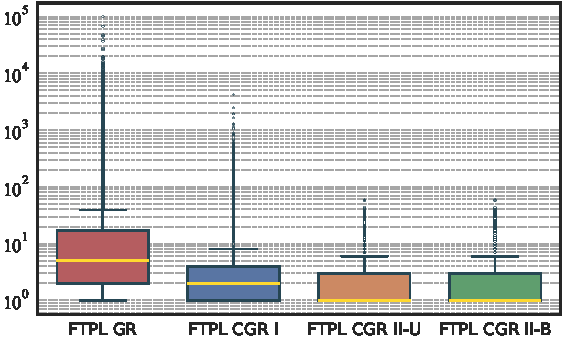
\includegraphics[width=\textwidth]{figures/boxplot_smallfig/box_32_sto.pdf} 
        \caption{Number of resampling for stochastic setting and $K=32$.}
        \label{fig:box_32_sto}
    \end{minipage}
    \begin{minipage}[c]{0.48\textwidth}
        \centering
        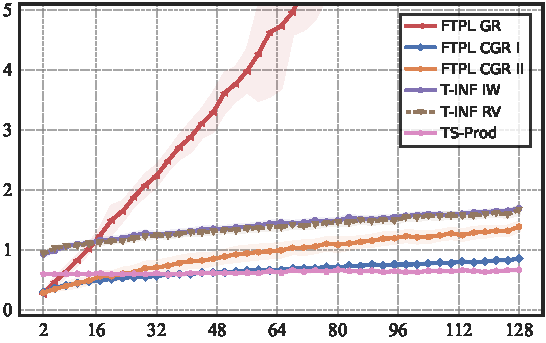
\includegraphics[width=\textwidth]{figures/runtime_sto_5.pdf} 
        \caption{Runtime (sec) for stochastic setting and different $K$.}
        \label{fig:runtime_sto}
    \end{minipage}
    \vskip 3mm
    \begin{minipage}[b]{\textwidth}
        \centering
        \begin{subfigure}[c]{0.4\textwidth}
            \centering
            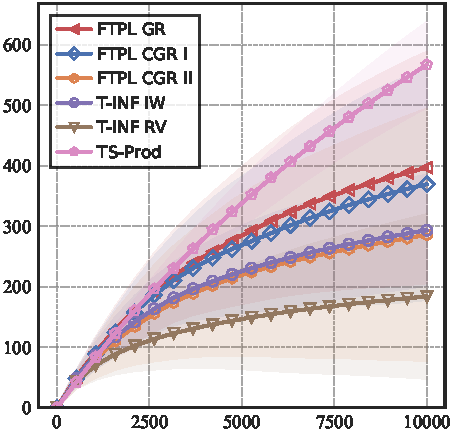
\includegraphics[width=\textwidth]{figures/regret_smallfig/s_6_na_8_d_8_dist_Ber_m_mab_nv_1.0.pdf}
            \caption{$K=8$}
            \label{fig:regret_8_sto}
        \end{subfigure}
        \begin{subfigure}[c]{0.4\textwidth}
            \centering
            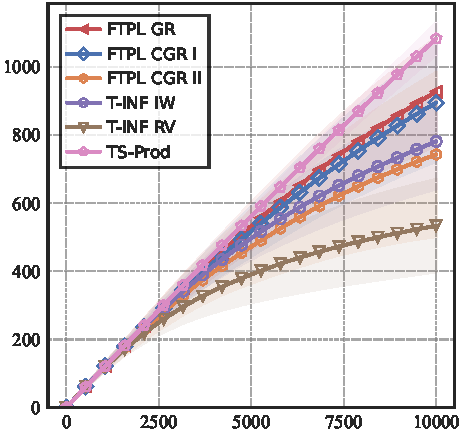
\includegraphics[width=\textwidth]{figures/regret_smallfig/s_6_na_32_d_32_dist_Ber_m_mab_nv_1.0.pdf}
            \caption{$K=32$}
            \label{fig:regret_32_sto}
        \end{subfigure}
        % \nextfloat
        \caption{Pseudo regret in stochastic setting.}
        \label{fig:regret_sto}
    \end{minipage}
\end{figure}

% In this appendix, we firstly describe the details of stochastic setting and stochastically constrained adversarial setting (or adversarial setting in short), and then provide results of additional experiments to complement those presented in Section~\ref{sect_exp}. 
In this appendix, we provide results of additional experiments to complement those presented in Chapter~\ref{sect_exp}. 

% \subsection{Details of Settings}
% In our experiments for both settings, the losses of each arms follow the Bernoulli distributions, and we exclusively consider the case where the suboptimality gap $\Delta=0.125$. For the stochastic setting, which is implemented for the experiments shown in Figures~\ref{fig:box_32_sto}, \ref{fig:runtime_sto}, \ref{fig:regret_sto}, \ref{fig:scatter_mean_32_sto} and \ref{fig:scatter_max_32_sto}, the mean losses are decided as $\qty(1-\Delta)/2$ for the single optimal arm and $\qty(1+\Delta)/2$ for the other suboptimal arms.

% For stochastically constrained adversarial setting, which is implemented for the experiments shown in Figures~\ref{fig:box_32_adv}, \ref{fig:runtime_adv}, \ref{fig:regret_adv}, \ref{fig:scatter_mean_32_adv} and \ref{fig:scatter_max_32_adv}, the mean losses for the single optimal arm and the suboptimal arms switch between $\qty(1-\Delta, 1)$ and $\qty(0, \Delta)$, with the duration of each phase growing exponentially by a factor of $1.6$ after every switch. Both settings are similar to those in \citet{JMLR:v22:19-753}.

% \subsection{Additional Results}
Consistently with the experiments in Chapter~\ref{sect_exp}, the results of $100$ trials are shown in this appendix.
% Figures~\ref{fig:box_32_sto}, \ref{fig:runtime_sto} and \ref{fig:regret_sto} 
Figures~\ref{fig:box_32_sto}--\ref{fig:regret_sto} 
show the results of the number of resampling, runtime and regret performance for stochastic setting, respectively.
They lead to the similar conclusions to those for the adversarial setting, that is, {\sf{FTPL~CGR}} not only effectively controls the number of resampling and significantly improves the runtime, but also achieves the better empirical regret performance, which seems to be due to the reduced variance of the loss estimator.
In addition, Figure~\ref{fig:scatter_32} provides a visualization of the average and maximum number of resampling at each round over $100$ trials for both settings, as a complement to the overview shown in Figures~\ref{fig:box_32_adv} and \ref{fig:box_32_sto}.
We can see that, under all the variants of {\sf{FTPL~CGR}}, the number of resampling at each round is stably controlled at a significantly low value, which is particularly pronounced for {\sf{FTPL~CGR~II}}.
Another interesting observation from Figures~\ref{fig:scatter_mean_32_adv} and \ref{fig:scatter_mean_32_sto} is that, for {\sf{FTPL~GR}} and {\sf{FTPL~CGR~I}}, the average number of resampling fluctuates within a range throughout the horizon, whereas that for {\sf{FTPL~CGR~II}} tends to be gradually reduced as the round progresses, seemingly due to the widening gap of the cumulative estimated losses between the arms.

\begin{figure}[htbp] 
    \centering
    \captionsetup[subfigure]{skip=0cm}
    \setlength{\belowcaptionskip}{0.2cm}
    \begin{subfigure}{\textwidth}
        \centering
        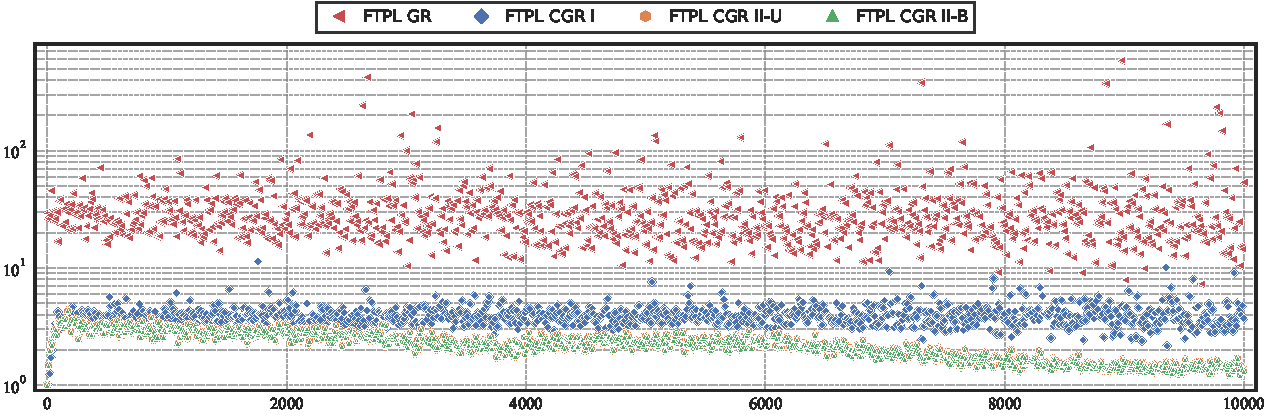
\includegraphics[width=0.94\textwidth]{figures/scatter/mt_mean_32_adv.pdf}
        \caption{Average, adversarial setting.}
        \label{fig:scatter_mean_32_adv}
    \end{subfigure}
    \hfill
    \begin{subfigure}{\textwidth}
        \centering
        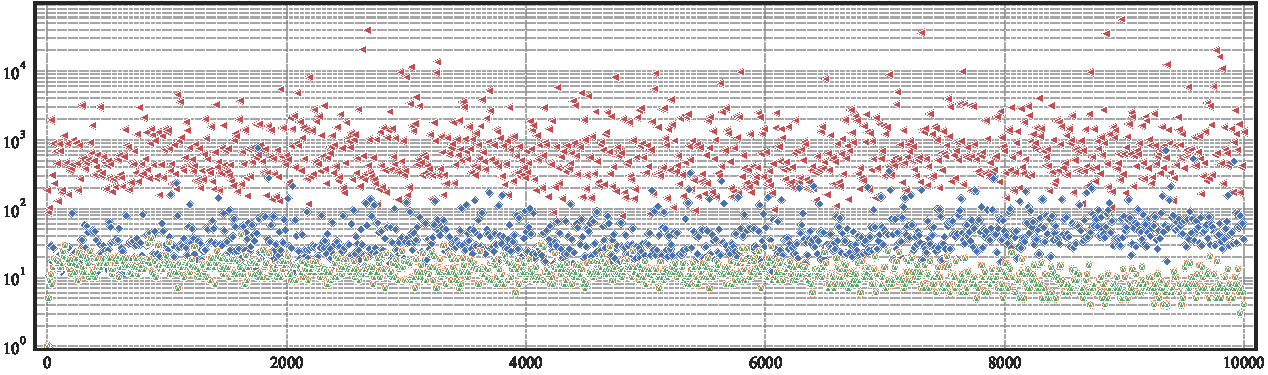
\includegraphics[width=0.94\textwidth]{figures/scatter/mt_max_32_adv_nolegend.pdf}
        \caption{Maximum, adversarial setting.}
        \label{fig:scatter_max_32_adv}
    \end{subfigure}
    \begin{subfigure}{\textwidth}
        \centering
        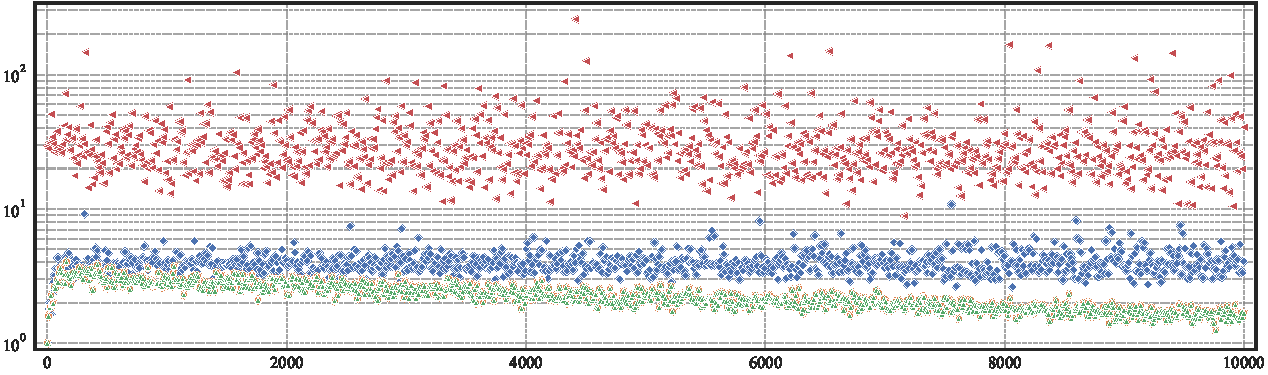
\includegraphics[width=0.94\textwidth]{figures/scatter/mt_mean_32_sto_nolegend.pdf}
        \caption{Average, stochastic setting.}
        \label{fig:scatter_mean_32_sto}
    \end{subfigure}
    \begin{subfigure}{\textwidth}
        \centering
        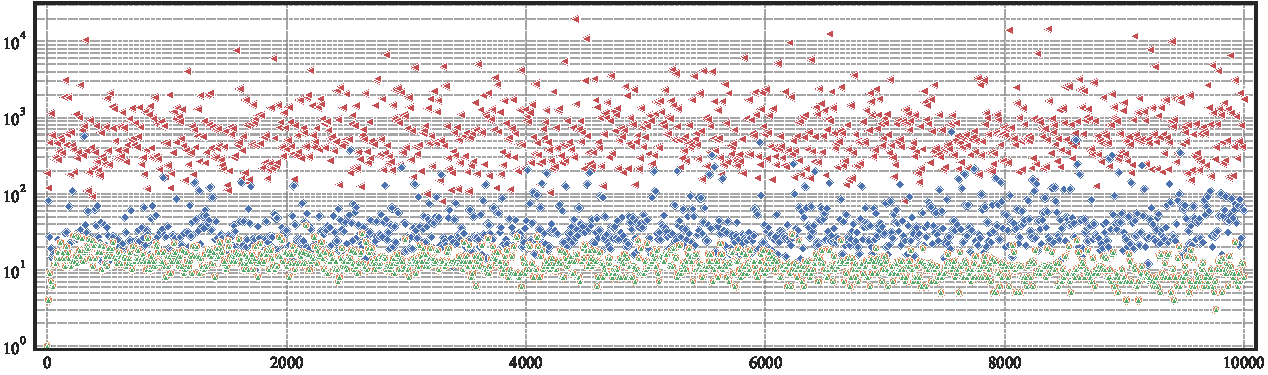
\includegraphics[width=0.94\textwidth]{figures/scatter/mt_max_32_sto_nolegend.pdf}
        \caption{Maximum, stochastic setting.}
        \label{fig:scatter_max_32_sto}
    \end{subfigure}
    \caption{Average or Maximum number of resampling at each round for $K=32$.}
    \label{fig:scatter_32}
\end{figure}